\documentclass[a4paper,14pt]{extarticle} \usepackage[utf8]{inputenc}
\usepackage[T1]{fontenc}
\usepackage[margin=2.5cm]{geometry}

% Fonte Caladea se existir, senão lmodern
\IfFileExists{caladea.sty}{
  \usepackage{caladea}
}{
  \usepackage{lmodern} }
\usepackage{ragged2e}
\usepackage{graphicx}
\usepackage[portuguese]{babel}
\usepackage{wrapfig}
\usepackage{hyperref}
\usepackage{fancyhdr}
\usepackage{xcolor}
\usepackage{rotating}
\usepackage{titlesec}
\usepackage{epigraph}
\usepackage{dirtytalk}
\usepackage{indentfirst} % Indenta o primeiro parágrafo após seções

% Ajuste do recuo de parágrafo
\setlength{\parindent}{1.5em}

% Adjust headheight to remove LaTeX warning
\setlength{\headheight}{17.54163pt}

% Centralizar títulos
\titleformat{\section}
  {\normalfont\centering\bfseries\Large}{}{1em}{}

\titleformat{\subsection}
  {\normalfont\centering\bfseries\large}{}{1em}{}

\titleformat{\subsubsection}
  {\normalfont\centering\bfseries}{}{1em}{}

% -------------- Símbolos de Versículo e Resposta --------------
% Definição do símbolo (a “barrinha” inclinada)
\makeatletter
\newcommand{\vers@resp@sym}{%
  \raisebox{0.2ex}{\rotatebox[origin=c]{-20}{$\m@th\rceil$}}%
}
% macro interna que sobrepõe a barrinha e a letra V ou R
\newcommand{\vers@resp}[2]{%
  {\ooalign{%
     \hidewidth\kern#1\vers@resp@sym\hidewidth\cr
     #2\cr
  }}%
}
% comandos públicos \versicle e \response
\DeclareRobustCommand{\versicle}{\vers@resp{-0.1em}{V}}
\DeclareRobustCommand{\response}{\vers@resp{0pt}{R}}
\makeatother
% ^------------- Símbolos de Versículo e Resposta -------------^

% Rodapé com imagem e página
\pagestyle{fancy}
% ---- Cabeçalho ------------
\fancyhf[C]{}
% ----- Rodapé --------------
\fancyfoot[C]{%
  
\includegraphics[scale=0.2]{assets/cross.png}\quad
  \textit{\textit{Beato Engelmar Uzeitig, Rogai por Nós}}\quad
  \thepage
}

\usepackage{pdfpages}
\begin{document}
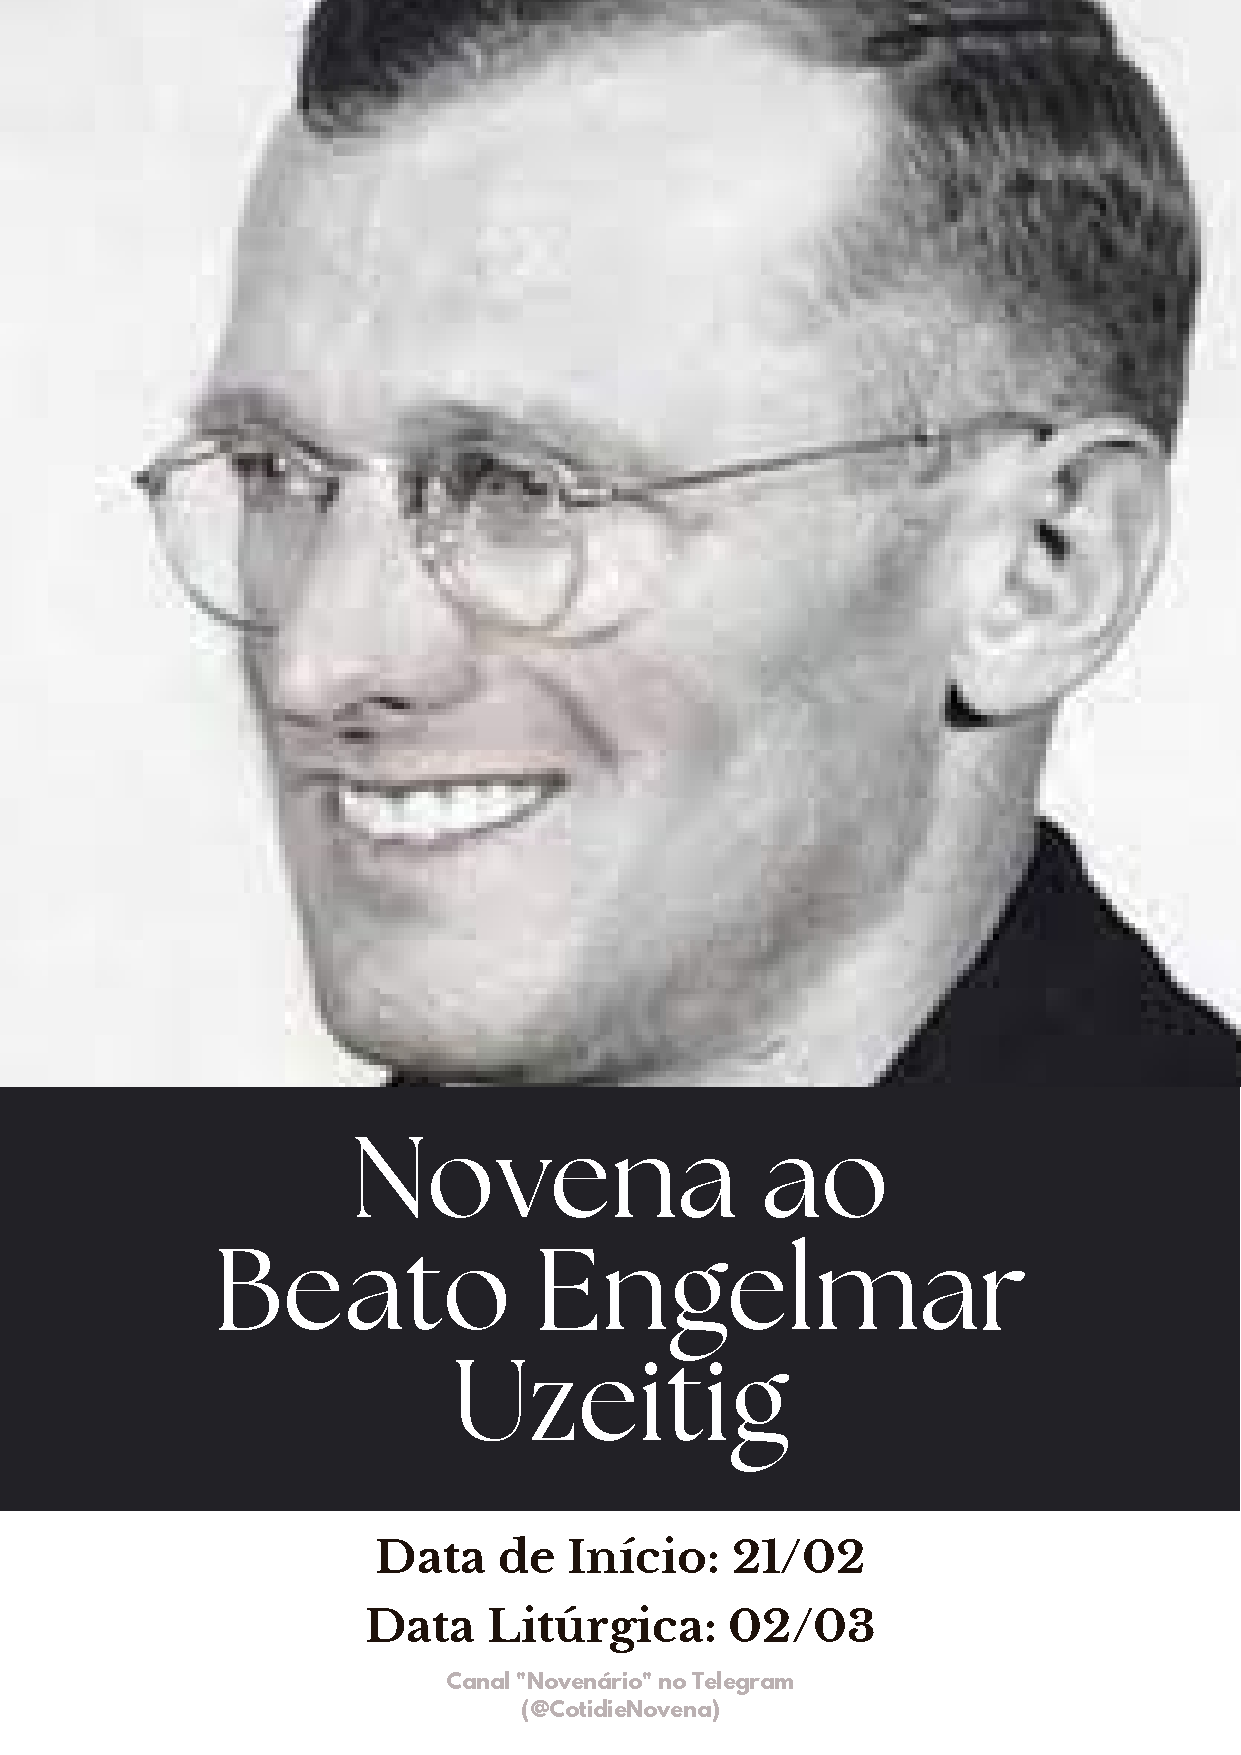
\includepdf[pages=1]{Capa Beato Engelmar}


\begin{center}
  {\huge Novena do Beato Engelmar}
\end{center}



\noindent\rule{\textwidth}{0.4pt}

\tableofcontents

\thispagestyle{empty}


% --- Origem ---
\newpage

\section{História}

\subsection{Quem foi o “Anjo de Dachau”}

Padre Engelmar Unzeitig, jovem sacerdote de origem tcheca foi preso pelos nazistas em 21 de abril de 1941.

A acusação que sobre ele recaia era de “pregar contra o Terceiro Reich, especialmente contra as medidas tomadas em relação ao povo judeu, como também por incentivar a sua Congregação a permanecer fiel a Deus e a resistir contra as mentiras do regime nazista”.

O sacerdote foi enviado para o Campo de extermínio alemão de Dachau, que era conhecido como “o maior mosteiro do mundo”: nele foram colocados como prisioneiros e ali martirizados cerca de 2.700 clérigos, dos quais 95% eram sacerdotes católicos poloneses, ali martirizados.

Padre Engelmar nasceu em 1911, em Greifendorf, na atual República Tcheca. Ele ingressou
no seminário da Sociedade Missionária Mariannhill aos 18 anos. Quando ele foi feito
prisioneiro pelos nazistas, em Dacau, tinha completado apenas dois anos de sacerdócio
e 30 anos de vida. Seu lema era: “Se ninguém mais for: eu vou!”.

\subsection{Prisão – Martírio – Apostolado e Serviço}

Depois de prisioneiro, Padre Engelmar estudou russo. Seu objetivo era de ajudar os que chegavam para aquele campo de extermínio vindos da Europa Oriental. Seu apostolado era o serviço ao demais e por isso foi considerado um “santo”, dentro do Campo de Dachau, era o “anjo”.

Naquela prisão, os religiosos eram tratados de modo “aleatório” e portanto imprevisível para os prisioneiros.

Por vezes, era-lhes permitido rezar. Porém, em outras ocasiões, por causa da prática de um pequeno ato de piedade, as punições eram severas, desumanas. Por uma dessas práticas feita numa Sexta-feira Santa, os nazistas selecionaram dezenas de sacerdotes e os torturaram.

\subsection{Caridade com os enfermos}

Apesar dos maus tratos e tudo o mais que se sofria naquela prisão, o Padre Engelmar tinha uma saúde que poderia se considerada boa.

Durante uma epidemia de febre tifoide que grassou pelo campo de concentração, ele e mais outros 19 sacerdotes se ofereceram como voluntários para atender aos doentes e moribundos.

Enquanto atendiam os doentes com esmero, corriam seriamente o risco de serem assassinados pois eles davam banho nos doentes, cuidavam e rezavam com eles e lhes administravam a unção dos enfermos. Atos arriscados que poderiam levá-los à morte.

\subsection{Testemunho e morte}

Dentro das duras circunstância em que sobrevivia em Dachau, o Beato Padre Engelmar encontrava tempo, esperança e alegria para praticar a sua fé. As cartas que ele escreveu a sua irmã testemunham testemunham sua atitude de vida católica, corajosa e santa.

Padre Engelmar Unzeitig morreu de febre tifóide junto com outros dois sacerdotes voluntários, em 2 de março de 1945. Algumas semanas depois de sua morte o campo de extermínio de Dachau foi liberado pelos soldados americanos que não puderam libertá-lo em tempo:

Ele já havia sido libertado antes, partira para a Casa do Pai. (JSG)

% --- Orações Diárias ---
\newpage

\vfill

\section{Orações}
\subsection{Oração Inicial}\label{sub:inicial} % (fold)

Senhor, nós vos agradecemos e louvamos por nos dar o Beato Engelmar como exemplo de Santidade. Por favor, ouça nossas orações por meio dele.

\subsection{Dia 1}

\underline{\nameref{sub:inicial}}

Caríssimo Senhor, nós vos agradecemos e vos louvamos por nos ter dado o Beato Engelmar Unzeitig como exemplo de santidade. Por favor, ouvi as suas orações em nosso nome! Beato Engelmar Unzeitig, ouviste o chamado de Deus para servi-lO no sacerdócio e na vida religiosa ainda jovem. Naquela época, havia muitas incertezas em tua vida e no mundo ao teu redor, pois a Segunda Guerra Mundial estava prestes a começar. Mas tu respondeste generosamente ao chamado de Deus para servi-lO.

Nós vos pedimos que leve os nossos pedidos ao Nosso Senhor, e de modo particular pedimos hoje que interceda por mais vocações ao sacerdócio e à vida religiosa. 

Rogai por nós, para que possamos servir a Deus tão de coração como tu o fizeste. Rogai para que possamos crescer em santidade e virtude em todas as oportunidades. E especialmente rezamos nesta novena por (mencione suas intenções aqui).

\underline{\nameref{sub:final}}

\subsection{Dia 2}

\underline{\nameref{sub:inicial}}

Beato Engelmar Unzeitig, aceitaste de bom grado o chamado de Deus para servi-lO no sacerdócio e como membro da Ordem Missionária de Mariannhill. Durante toda a tua vida, continuaste a te submeter à vontade de Deus. Mantiveste tua devoção a Ele mesmo no meio de sofrimentos horríveis e morte.

Pedimos que leve nossos pedidos ao Nosso Senhor e, em particular, pedimos hoje que reze para que possamos crescer na submissão à vontade de Deus em nossas vidas. 

Rogai por nós para que possamos imitar o vosso santo exemplo em nossas próprias vidas. Rezai para que possamos realmente nos esforçar para nos tornarmos santos, mesmo em meio ao sofrimento. E pedimos especialmente nesta novena por (mencione suas intenções aqui).


\underline{\nameref{sub:final}}

\subsection{Dia 3}

\underline{\nameref{sub:inicial}}

Beato Engelmar Unzeitig, escolheste servir a Deus de forma plena como sacerdote em Sua Igreja. Durante o teu ministério sacerdotal, trabalhaste para pregar a verdade e para ministrar ao povo de Deus. Mesmo no meio de sofrimentos horríveis, permaneceste firme no teu amoroso serviço sacerdotal.

Pedimos que leves nossas intenções ao Nosso Senhor, e pedimos especialmente hoje que reze para que Deus abençoe e assista a todos os sacerdotes. 

Rogai por nós, para que possamos sempre estar prontos a servir a Deus em todas as formas que Ele nos chamar. Rezai para que possamos crescer em devoção a cada dia de nossas vidas. E especialmente rezamos nesta novena por (mencione suas intenções aqui).


\underline{\nameref{sub:final}}

\subsection{Dia 4}

\underline{\nameref{sub:inicial}}

Beato Engelmar Unzeitig, sentiste o chamado de Deus para servi-lO como sacerdote e como membro da Ordem Missionária de Mariannhill.
Enquanto trabalhavas para servir o povo de Deus,
 pregaste e defendeste a verdade destemidamente,
 mesmo sabendo que isso poderia custar tua vida nas mãos dos nazistas.

Pedimos que leves nossos pedidos ao Nosso Senhor, e pedimos particularmente hoje que reze para que Deus abençoe e assista todos os pregadores. 

Rogai por nós, para que possamos sempre ser destemidos em pregar o Evangelho. Rezai para que possamos sempre fazer tudo que estiver ao nosso alcance para trazer almas a Deus. E especialmente rezamos nesta novena por (mencione suas intenções aqui).


\underline{\nameref{sub:final}}

\subsection{Dia 5}

\underline{\nameref{sub:inicial}}

Beato Engelmar Unzeitig, corajosamente proclamaste a verdade em tuas homilias, mesmo sabendo que isso poderia te tornar um alvo da perseguição nazista. Durante o teu tempo no campo de concentração, continuaste a praticar tua fé corajosamente, em meio a perigos e sofrimentos.

Pedimos que leves nossos pedidos ao Nosso Senhor, e pedimos particularmente hoje que intercedas para que Deus nos ajude e a todas as pessoas a crescerem em santa coragem. 

Rogai por nós, para que possamos crescer em todas as virtudes necessárias para a santidade. Rogai para que sempre façamos o que for necessário para avançar em santidade e servir dignamente a Deus. E especialmente rezamos nesta novena por (mencione suas intenções aqui).


\underline{\nameref{sub:final}}

\subsection{Dia 6}

\underline{\nameref{sub:inicial}}

Beato Engelmar Unzeitig, foste enviado ao campo de concentração de Dachau sem sequer um julgamento, porque proclamaste a verdade e defendeste os judeus. Enquanto sofrias imensamente no campo de concentração, serviste teus companheiros de prisão com o melhor de tua capacidade, por amor a Deus.

Pedimos que leves nossas intenções ao Nosso Senhor, e pedimos particularmente hoje que reze para que Deus nos ajude e a todas as pessoas a crescerem na verdadeira caridade. 

Rogai por nós, para que possamos sempre servir nossos irmãos e irmãs por amor a Deus. Rogai para que nunca percamos a oportunidade de praticar a virtude em nossas vidas. E especialmente rezamos nesta novena por (mencione suas intenções aqui).


\underline{\nameref{sub:final}}

\subsection{Dia 7}

\underline{\nameref{sub:inicial}}

Beato Engelmar Unzeitig, suportaste intenso sofrimento durante o teu encarceramento no campo de concentração de Dachau. Mas, apesar de tudo o que estavas a sofrer, perseveraste em servir a Deus e em praticar a virtude heroica. Não permitiste que nenhum dos teus sofrimentos te impedisse de perseverar na santidade.

Pedimos que leves nossas intenções ao Nosso Senhor, e pedimos particularmente hoje que reze para que Deus nos ajude e a todas as pessoas a crescerem em perseverança. 

Rogai por nós, para que possamos sempre fazer tudo o que pudermos para avançar na santidade em cada dia. Rogai para que possamos encontrar forças para praticar a virtude mesmo em meio ao sofrimento. E especialmente rezamos nesta novena por (mencione suas intenções aqui).

\underline{\nameref{sub:final}}

\subsection{Dia 8}

\underline{\nameref{sub:inicial}}

Beato Engelmar Unzeitig, foste preso por pregar a verdade e defender os judeus contra a perseguição nazista. Foste enviado ao campo de concentração de Dachau, onde sofreste muito nas mãos daqueles que odiavam a fé católica.

Pedimos que leves nossas intenções ao Nosso Senhor, e pedimos particularmente hoje que reze para que Deus fortaleça e assista todos os que estão sendo perseguidos pela fé em nosso mundo moderno. 

Rogai por nós, para que sempre sejamos corajosos em praticar nossa fé, não importando o quão difícil isso possa ser. Rogai para que coloquemos sempre o amor a Deus acima de tudo em nossas vidas. E especialmente rezamos nesta novena por (mencione suas intenções aqui).


\underline{\nameref{sub:final}}

\subsection{Dia 9}

\underline{\nameref{sub:inicial}}

Beato Engelmar Unzeitig, sofreste grandemente durante o teu encarceramento no campo de concentração de Dachau. Apesar das tuas muitas dores, nunca vacilaste na tua fé. Em vez disso, o teu amor por Deus cresceu mais profundo à medida que trabalhavas para servi-Lo e oferecer os teus sofrimentos a Ele.

Pedimos que tragas as nossas intenções diante do Nosso Senhor, e pedimos particularmente hoje que reze para que Deus nos ajude e a todas as pessoas a crescer na capacidade de unir nossos sofrimentos aos Dele!

Rogai por nós, para que possamos servir a Deus mais profundamente em cada dia de nossas vidas. Rogai para que possamos avançar em santidade e virtude mesmo em meio às grandes dificuldades. E especialmente rezamos nesta novena por (mencione suas intenções aqui).
    
\underline{\nameref{sub:final}}

\subsection{Oração Final}\label{sub:final} % (fold) \subsection{Orações de Cada Dia}

\[\textbf{Pai-Nosso, Ave-Maria, Glória}\]


\vfill

\begin{center}
\subsection*{Fontes:}
Adaptado de: {\color{blue} \underline{\href{https://gaudiumpress.org/content/82365-padre-engelmar-unzeitig-o-anjo-de-dachau-foi-beatificado/}{Gaudium Press}}} e {\color{blue} \underline{\href{https://www.praymorenovenas.com/blessed-engelmar-unzeitig-novena}{Pray More Novenas}}}
\end{center}


\end{document}
